\documentclass[12pt
,headinclude
,headsepline
,bibtotocnumbered
]{scrartcl}
\usepackage[paper=a4paper,left=25mm,right=25mm,top=25mm,bottom=25mm]{geometry} 
\usepackage[utf8]{inputenc}
\usepackage[english]{babel}
\usepackage{fancyvrb}  % Add this line
\usepackage{graphicx}
\usepackage{multirow}
\usepackage{pdfpages}
%\usepackage{wrapfig}
\usepackage{placeins}
\usepackage{float}
\usepackage{flafter}
\usepackage{mathtools}
\usepackage{hyperref}
\usepackage{epstopdf}
\usepackage[miktex]{gnuplottex}
\usepackage[T1]{fontenc}
\usepackage{mhchem}
\usepackage{fancyhdr}
%\setlength{\mathindent}{0pt}
\usepackage{amssymb}
\usepackage[list=true, font=large, labelfont=bf, 
labelformat=brace, position=top]{subcaption}
\setlength{\parindent}{0mm}
\usepackage{listings}
\usepackage{color}

\definecolor{dkgreen}{rgb}{0,0.6,0}
\definecolor{gray}{rgb}{0.5,0.5,0.5}
\definecolor{mauve}{rgb}{0.58,0,0.82}

\lstset{ %
	language=Python,                % the language of the code
	basicstyle=\small\ttfamily,     % the size of the fonts that are used for the code
	numbers=left,                   % where to put the line-numbers
	numberstyle=\tiny\color{gray},  % the style that is used for the line-numbers
	stepnumber=1,                   % the step between two line-numbers. If it's 1, each line will be numbered
	numbersep=5pt,                  % how far the line-numbers are from the code
	backgroundcolor=\color{white},  % choose the background color. You must add \usepackage{color}
	showspaces=false,               % show spaces adding particular underscores
	showstringspaces=false,         % underline spaces within strings
	showtabs=false,                 % show tabs within strings adding particular underscores
	frame=single,                   % adds a frame around the code
	rulecolor=\color{black},        % if not set, the frame-color may be changed on line-breaks within not-black text (e.g. commens (green here))
	tabsize=2,                      % sets default tabsize to 2 spaces
	captionpos=b,                   % sets the caption-position to bottom
	breaklines=true,                % sets automatic line breaking
	breakatwhitespace=true,         % sets if automatic breaks should only happen at whitespace
	title=\lstname,                 % show the filename of files included with \lstinputlisting; also try caption instead of title
	keywordstyle=\color{blue},      % keyword style
	commentstyle=\color{dkgreen},   % comment style
	stringstyle=\color{mauve},      % string literal style
	escapeinside={\%*}{*)},         % if you want to add LaTeX within your code
	morekeywords={*,...}            % if you want to add more keywords to the set
}

\setlength{\parindent}{0mm}

\pagestyle{fancy}
\fancyhf{}
\lhead{PRE-T\\ Exercise 2: Sampling and Filters }
\rhead{Hsin-Feng Ho \\03770686}
\rfoot{Page \thepage}	
\begin{document}
\section{Sampling - Coordinate systems}
An orthophoto of English Garden in Munich with a pixel resolution of 0.4 m is given.
Firstly we have to complete the funcion $subset$ in ordert to extract the subset of the image. The function is shown in the following code.
\begin{lstlisting}
    def subset(I, x, y, nu, nv):
    p_ul = (x,y) # tuple with img coord. upper left corner
    p_lr = (x+nu,y+nv) # tuple with img coord. lower right corner
    
    S = I[p_ul[1] : p_lr[1], p_ul[0] : p_lr[0] , :] # subset S with all channels (:)
    return S
\end{lstlisting}
The function $subset$ takes the image $I$ and the coordinates of the upper left corner $(x,y)$ and the lower right corner $(x+nu,y+nv)$ of the subset as input. The function returns the subset $S$ of the image $I$.
\\\\
A subset of the image is shown in Figure \ref{fig:main}. The subset is the area of the English Garden in Munich. The subset is extracted from the image with the function $subset$.
\begin{figure}[H]
    \centering
    \begin{subfigure}{0.45\textwidth}
        \centering
        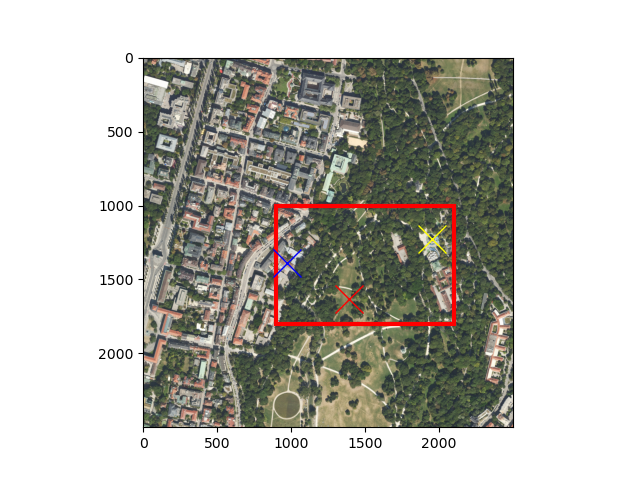
\includegraphics[width=1.5\textwidth]{ex02_task1_1.png}
        \label{fig:sub1}
    \end{subfigure}
    \hfill
    \begin{subfigure}{0.45\textwidth}
        \centering
        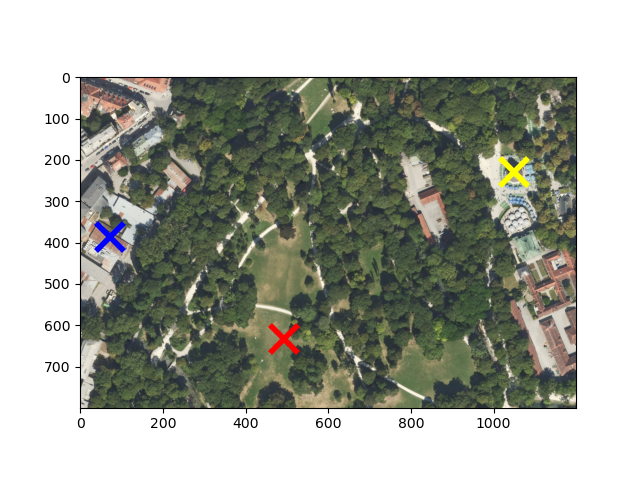
\includegraphics[width=1\textwidth]{ex02_task1_2.png}
        \label{fig:sub2}
    \end{subfigure}
    \caption{Subset of the image}
    \label{fig:main}
\end{figure}
We also have to calculate the UTM coordinates of the three points in the subset. The coordinates of the low right corner of the image is given. The coordinates of the three points are calculated with the scale and translation. The results are shown in the following. 
\begin{verbatim}
    p1_world:  [ 692780.  5336508.4]
    p2_world:  [ 692388.8 5336445.2]
    p3_world:  [ 692557.2 5336346.8]
\end{verbatim}
\section{Median and Mean}
In the first part of this exercise we have to implement the functions $median$ in order to calculate the median of a chess board like image. The function is shown in the following code.
\begin{lstlisting}
    def median(listValues):
    median_value = 0.0
    if len(listValues) == 2:
        raise ValueError('Number of values must be odd')
    else:
        listValues.sort()
        median_value = listValues[int(len(listValues)/2)]
    return median_value
\end{lstlisting}
And we have to calculate the mean and median for the following list of values: [19.7, 556.3, 23.2, 27.5, 16.3, 21.0, 27.2, 495.0, 25.3]. The results are shown in the following code.
\begin{verbatim}
    Mean:  134.61111111111111
    Median:  25.3
\end{verbatim}
\section{Filters}
In the second part of this exercise we have to use the mean filter and median filter to filter the chess board like image. The results are shown in Figure \ref{fig:mean}. 
\begin{figure}[H]
    \centering
    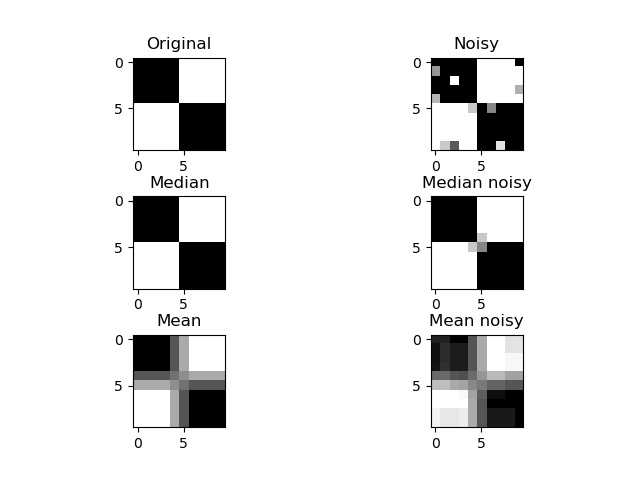
\includegraphics[width=0.8\textwidth]{chessboard.png}
    \caption{Mean and median filter}
    \label{fig:mean}
\end{figure}
From the results we can see that the mean filter is not able to remove the noise in the image. However, the median filter is able to remove the noise in the image. The reason is that the median filter is more robust to outliers than the mean filter. And the mean filter will blur the image. If we want to remove the noise in the image, we should use the median filter. If we want to blur the image, we should use the mean filter.
\\\\
There are other thechniques to perform the expanding of the image before applying the convolution. For example, we can use the zero padding to expand the image. The advantage of the zero padding is that it is easy to implement. The disadvantage of the zero padding is that it will introduce the artifacts in the image. Another example is the mirror padding. The advantage of the mirror padding is that it will not introduce the artifacts in the image. The disadvantage of the mirror padding is that it is difficult to implement. The other posibility is the replicate padding. It's similar to the mirror padding, which will not introduce the artifacts in the image. However, it is also difficult to implement.
\section{Sobel and Laplace filter}
In the third part of this exercise we have to implement the Sobel filter and Laplace filter. The results are shown in Figure \ref{fig:sobel} and Figure \ref{fig:laplace}.

\begin{figure}[H]
    \centering
    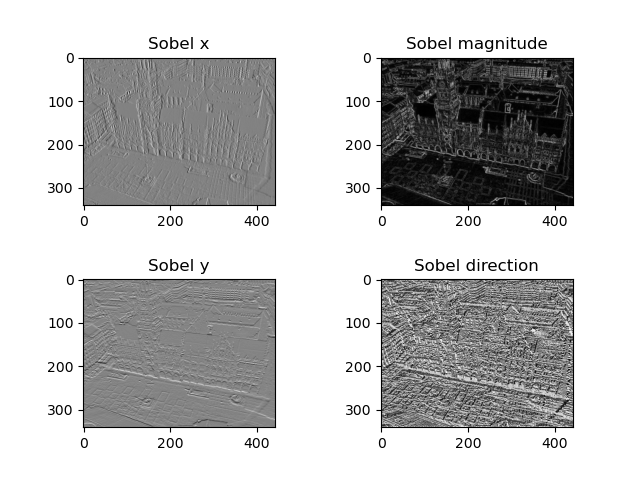
\includegraphics[width=1\textwidth]{sobel.png}
    \caption{Sobel filter}
    \label{fig:sobel}
\end{figure}
\begin{figure}[H]
    \centering
    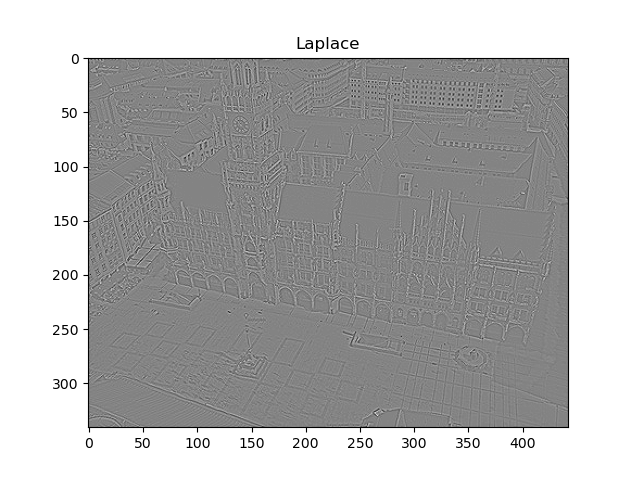
\includegraphics[width=0.6\textwidth]{laplace.png}
    \caption{Laplace filter}
    \label{fig:laplace}
\end{figure}
We have first to define the kernel of the Sobel filter and Laplace filter. 
\begin{align*}
    \text{Sobel filter x: } & \begin{bmatrix}
        -1 & 0 & 1 \\
        -2 & 0 & 2 \\
        -1 & 0 & 1
    \end{bmatrix} \\
    \text{Sobel filter y: } & \begin{bmatrix}
        -1 & -2 & -1 \\
        0 & 0 & 0 \\
        1 & 2 & 1
        \end{bmatrix} \\
    \text{Laplace filter: } & \begin{bmatrix}
        0 & 1 & 0 \\
        1 & -4 & 1 \\
        0 & 1 & 0
    \end{bmatrix}
\end{align*}
The calculation of magnitude and direction of the gradient is shown in the following code.
\begin{lstlisting}
    Smag = np.sqrt(Sx**2 + Sy**2)
    Sdir = np.arctan2(Sy,Sx)
\end{lstlisting}
The Sobel filter and Laplace filter are both used for edge detection in an image. The Sobel filter is a discrete differentiation operator. It is used to compute an approximation of the gradient of the image intensity function. The Laplace filter is a second order derivative edge detector. It is used to find the zero crossings in the second derivative of the image intensity function.  
\newpage
\section*{Code}
\lstinputlisting[language=Python,breaklines=true]{ex02_task1.py}
\lstinputlisting[language=Python,breaklines=true]{ex02_task2_3.py}
\end{document}